\documentclass{beamer}
\DeclareFontShape{OT1}{cmss}{b}{n}{<->ssub * cmss/bx/n}{} 
\usetheme{CambridgeUS}
\usecolortheme{rose}
\usepackage{amsmath}
\usepackage{amsfonts}
\usepackage{mathbbol}
\usepackage{xcolor} % before tikz or tkz-euclide if necessary
\usepackage{tkz-euclide} % no need to load TikZ
\usepackage{multirow}
\usepackage{lmodern}
\usepackage{bm}
\usepackage{subcaption}
%\usepackage{subfigure}

\usepackage[
backend=biber,
style=authoryear-icomp,
sortlocale=de_DE,
natbib=true,
url=false, 
doi=true,
eprint=false
]{biblatex}
\addbibresource{../Bibliography/main_JC.bib}



\titlegraphic{
\includegraphics[width=2cm]{../Figures/UAMS_RGB.png}
}


\title{Connectomics: Null Hypotheses}
\author{Horacio G\'omez-Acevedo}

\begin{document}

	\begin{frame}[plain]
		\maketitle
	\end{frame}

	\begin{frame}{Today's paper}
		\begin{figure}[h]
			\centering
			%	\begin{subfigure}{0.4\textwidth}
				%		\centering
				
\includegraphics[scale=0.45]{../Figures/fig_null_models_paper.png}
				%	\end{subfigure}
		\end{figure}
	\end{frame}
	
	
	\begin{frame}{Main Ideas}
	\begin{itemize}
		\item Rigorous identification and quantification of functionally important features of the brain network architecture.
		\item Using Null models for the presence and relevance of features (sensitivity analysis).
		\item Feature randomization (or bootstraping) to formally investigate relevance.
		\item Multiple null models are possible.
	\end{itemize}
		
	\end{frame}
	
	
	\begin{frame}{Features of Interest}
		Research on imaging across species have "reconstructed" graph organization of brain networks and have determined that:
		\begin{itemize}
			\item Connection profiles
			\item Degree distribution of nodes is heavy tailed ("few hyper-connected nodes")
			\item Densely interconnected network modules
		\end{itemize}
		How to determine the importance of features of interest (FOI)?
		\textbf{Null models} provide a way to systematically compare networks and reveal the presence of a FOI arises as a consequence of other features.
		
		What are network (graph) features?
		\begin{enumerate}
			\item Density, which refers to the proportion of edges.
			\item Degree sequence, which refers to the number of edges incident on each node
			\item Topology 
		\end{enumerate}
		 		
	\end{frame}
	
	\begin{frame}{Null Distribution}
		\begin{figure}[h]
			\centering
			%	\begin{subfigure}{0.4\textwidth}
				%		\centering
				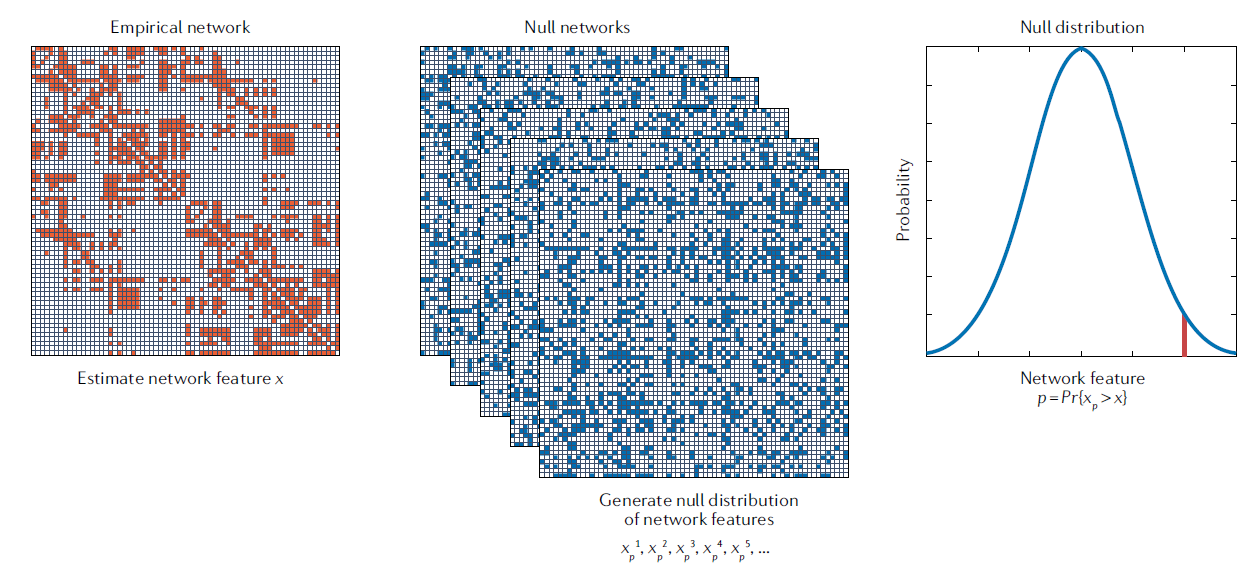
\includegraphics[scale=0.4]{../Figures/fig_null_models_1.png}
				%	\end{subfigure}
		\end{figure}
		
		I
	\end{frame}
	
	\begin{frame}{Graph Null networks}
		We begin with a network feature $F_I$ (e.g., path length) and an empirical network (adjacency matrix).
		
		
		We generate a population of null networks  by randomizing other feature $F_J$ (e.g., topology) and calculating the same feature $F_I$ for each of the randomized variants $F_I^{J_1},F_I^{J_2},\ldots$
		
		Generate the distribution of $\{F_I^{J_k}\}$. The corresponding hypothesis test 
		\begin{equation*}
			H_0\colon F_I=F_I^0 \qquad H_1\colon F_I>F_I^0
		\end{equation*}
		If you calculate the $p$-value associated with the feature $F_I$ distribution. 
		
		"construct a distribution of
		features $\{F_I^{J_k}\}$ under the null hypothesis that the magnitude of feature $F_I^0$ is due
		to properties that were preserved, and not due to properties that were
		randomized (and not preserved)"
		
	\end{frame}
	
	\begin{frame}{Randomization }
		
		A frequently used method is \textit{rewiring} in which pairs of edges are selected at random and then swapped. 
		
		
		\begin{figure}[h]
			\centering
			%	\begin{subfigure}{0.4\textwidth}
				%		\centering
				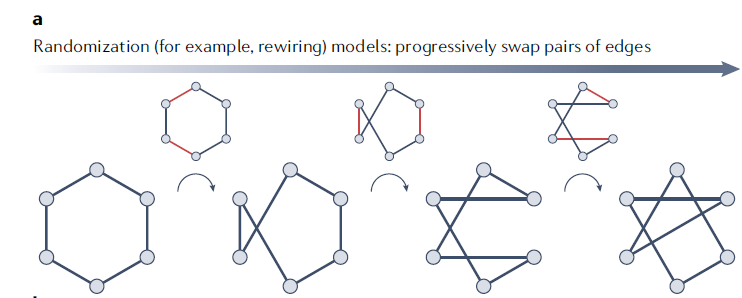
\includegraphics[scale=0.6]{../Figures/fig_null_models_2.png}
				%	\end{subfigure}
		\end{figure}
	\end{frame}
	
	\begin{frame}{Generative Models}
		These models \textit{build} the network using a predefined wiring rule that embodies the null hypothesis. This process stops when the network has the same size and density as the observed one.
		\begin{figure}[h]
			\centering
			%	\begin{subfigure}{0.4\textwidth}
				%		\centering
				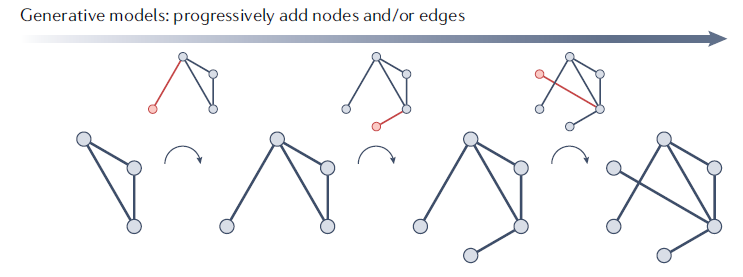
\includegraphics[scale=0.5]{../Figures/fig_null_models_2b.png}
				%	\end{subfigure}
		\end{figure}	
	\end{frame}
	
	\begin{frame}{Other uses of Generative Models}
		
		These models have been also used for \textbf{model identification} or \textbf{model comparison}.
		
		As long as you have a \textbf{cost function}, the generative models produce a way to select an optimal solution.
		
		"This is conceptually similar to
		model identification in formulations of brain networks
		as dynamic systems, such as dynamic causal modelling,
		in which competing accounts of dynamic neural circuit
		interactions are tested to identify the best- fitting or
		most parsimonious model, or when competing hypotheses
		are grouped into distinct families of mechanisms
		or families of models"
		
	\end{frame}
	
	\begin{frame}{Null after null...}
		
		"An important methodological question
		is whether null models uniformly sample the target
		space. The mere fact that a model retains one feature
		and randomizes
		another does not mean that it samples
		the space of all possible realizations exhaustively. "
		\begin{figure}[h]
			\centering
			%	\begin{subfigure}{0.4\textwidth}
				%		\centering
				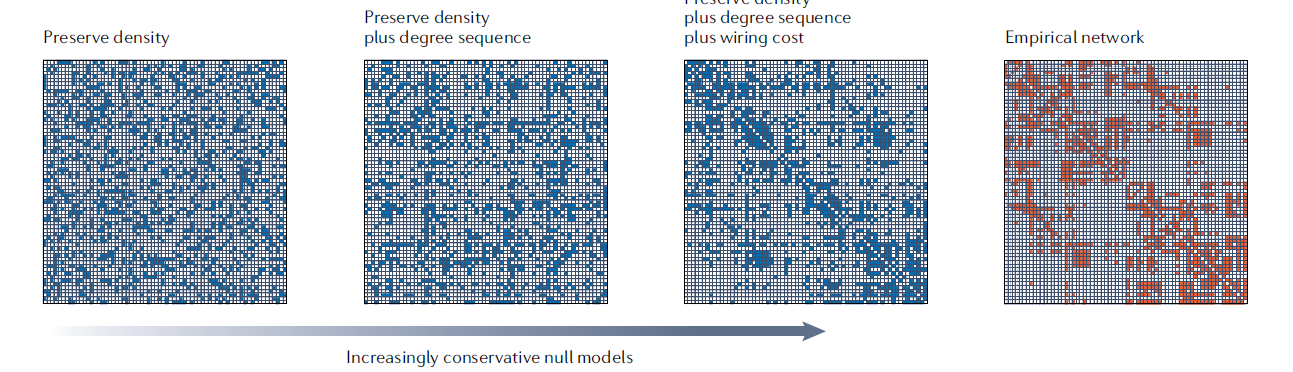
\includegraphics[scale=0.4]{../Figures/fig_null_models_3.png}
				%	\end{subfigure}
		\end{figure}	
	\end{frame}
\begin{frame}{Null after null... (cont)}	

	"Ultimately, there is no right or wrong null model. The
	null model should be an implementation of an explicit
	and falsifiable null hypothesis that is specific to one’s
	research question."
	
	
\end{frame}
	
	\begin{frame}{Null models for spatial networks}
		
		"Perhaps the most important feature to consider when
		analysing brain network topology is geometry"
		
		The challenge is the bias in connectivity between "close" neural elements.
		
		Also, the standard rewiring with naive swapping algorithm tend to form networks with unrealistic (and costly) configurations. 
		
		One possible alternative is to use \textbf{spatially repositioned nulls} that preserve topology but allow locations to be permuted. 
		
		"Collectively, geometric nulls enable us to quantify the
		proportion of topology that comes passively from spatial
		embedding"
		
	\end{frame}
\begin{frame}{Annotated networks (multi-omics)}
	"A typical comparison may
	involve correlating, across brain regions, a region’s
	network attribute (such as degree) and its microscale
	annotation (such as gene expression)"
	
	\textbf{We are violating independence!}
	
	"However, an important problem arises when
	estimating a p value for the correlation coefficient.
	Namely, the standard parametric method assumes that
	the two vectors come from an uncorrelated bivariate
	normal distribution, whereas the non- parametric (naive
	permutation- based) method assumes that the elements
	of the vectors are exchangeable. This independence
	assumption is violated by multiple forms of dependence
	between data points"

\end{frame}
\begin{frame}{Problems with independence}	
	\begin{itemize}
		\item Spatial autocorrelation. Similar values of anatomical
	and physiological measurements between neighbouring
	locations. 
	\item Homotopic symmetry. Similar measurements between corresponding locations
	within the left and right hemispheres of the brain. 
	\item Spatial resolution. The effect size on the
	number of regions, vertices or voxels.
	\end{itemize}
	
\end{frame}

\begin{frame}{Spin Test}
	\begin{figure}[h]
		\centering
		%	\begin{subfigure}{0.4\textwidth}
			%		\centering
			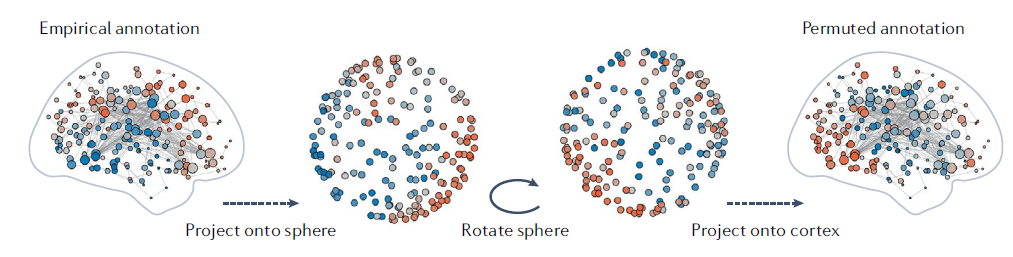
\includegraphics[scale=0.5]{../Figures/fig_null_models_5.png}
			%	\end{subfigure}
	\end{figure}	
\end{frame}

\begin{frame}{Correlation Networks}
	Connectivity is often measured with covariances. Thus, these networks are subject to transitivity issues.
	
	If node $A$ is positively correlated with nodes $B$ and $C$, nodes $B$ and $C$ may be negatively correlated. 
	
	We can randomize the signal itself:
	
	"surrogate time series can be
	generated by transforming empirical time series to the
	frequency domain using the Fourier transform, shuffling
	the phase coefficients and taking the inverse transform
	to the time domain. The resulting surrogate time series
	have preserved power spectra but randomized temporal
	dependencies" 
	
	\href{https://www.thefouriertransform.com/}{See this link for Fourier Transform}
\end{frame}
\begin{frame}{Randomization on steroids}
	\begin{figure}[h]
		\centering
		%	\begin{subfigure}{0.4\textwidth}
			%		\centering
			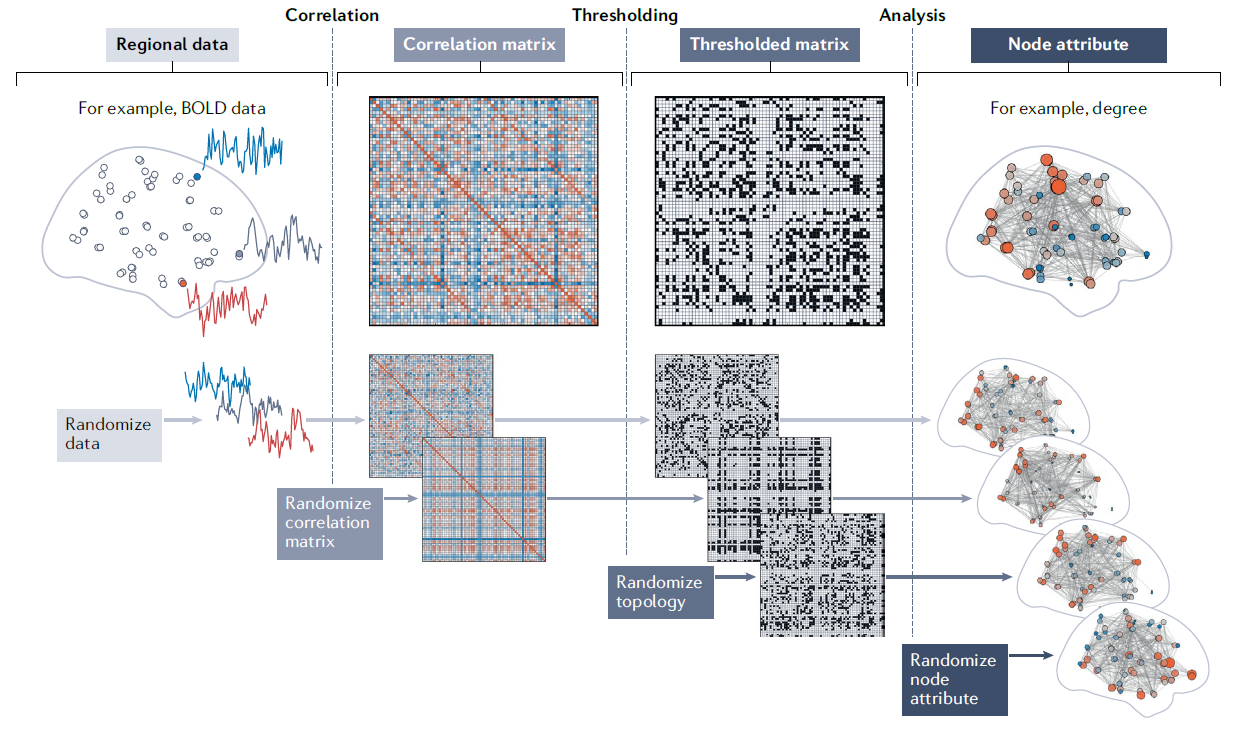
\includegraphics[scale=0.4]{../Figures/fig_null_models_6.png}
			%	\end{subfigure}
	\end{figure}	
\end{frame}
\begin{frame}{Conclusion}
	"In network neuroscience, null networks
	are typically created through complete randomization,
	and, conversely, generative models are typically fully
	completed. However, both processes can be paused
	incrementally to explore the immediate vicinity of an
	empirical network in null- model space, thereby giving
	insight into the stochastic neighbourhood of brain networks.
	Such ‘connectome mutagenesis’ can offer insight
	into pathological perturbations involved in psychiatric
	and neurological disorders"
\end{frame}
%-----------------------------	
\section{Introduction to Hypothesis Testing}	
\begin{frame}{Hypothesis Testing}
	There are key components to take full advantage of th
	
	\begin{itemize}
		\item Likelihood
		\item Statistical Hypothesis
		\item Hypothesis Test
		\item Likelihood Ratio
		\item Asymptotic Properties of the Normal Distribution
		\item $p$-values
	\end{itemize}
\end{frame}
\begin{frame}{Likelihood}
	If we have $X_1,\ldots, X_n$ independent and identically distributed (iid) random variables with a common probability (mass/density) function $f(x;\theta)$ where the parameter $\theta$ is unknown ($\theta \in \Omega$). The likelihood of a sample $\vec{x}=(x_1,\ldots,x_n)$ is 
	\begin{equation*}
		L(\theta,\vec{x})= \prod_{i=1}^n f(x_i,\theta)
	\end{equation*}
	Example: If we have $X_i \sim N(\theta,\sigma^2)$ with $\sigma^2>0$ known but $\theta$ unknown. Then
	\begin{equation*}
		L(\theta,\vec{x})= \left(\frac{1}{2\pi \sigma^2}\right)^{n/2}
		\exp\left(- \frac{1}{2\sigma^2}\sum_{i=1}^n (x_i-\overline{x})^2\right)\exp\left(- \frac{1}{2\sigma^2}n(\overline{x}-\theta)^2\right)
	\end{equation*}
\end{frame}

\begin{frame}{Statistical Hypothesis}
	A Statistical Hypothesis is a conjecture about the probability distribution of a population. 
	
	Example: We suppose that in an experiment we have a random sample from $N(\theta,10)$. 
	\begin{equation*}
		\begin{split}
			H_0 &\colon \text{ The population is } N(5,10) \text{-distributed}\\
			H_1 &\colon \text{ The population is } N(1,10) \text{-distributed}
		\end{split}
	\end{equation*}
\end{frame}

\begin{frame}{Hypothesis Test}
	A Hypothesis Test is a tuple $(X_1,\ldots, X_n; H_0,H_1,G)$, where
	\begin{enumerate}
		\item $(x_1,\ldots, x_n)$ is a sample of $(X_1,\ldots, X_n)$ random variables iid.
		\item $H_0$ and $H_1$ are hypothesis concerning the probability distribution of the population.
		\item $G\subset \mathbb{R}^n$ is Borel set (countable unions of open sets). 
	\end{enumerate}
	The \textbf{level of significance} is defined as 
	\begin{equation*}
		\alpha = P^{H_0}_{X_1,\ldots, X_n}(G)
	\end{equation*}
	We will consider hypothesis such as
	\begin{equation*}
		H_0\colon \theta=\theta_0 (\text{ or }\theta \in \Theta_0) \qquad H_1 \colon \theta\ne \theta_0 (\text{ or }\theta \in \Theta=\Theta_1\cup \Theta_0)
	\end{equation*}
	
\end{frame}

\begin{frame}{Maximum Likelihood Test}
	The \textbf{likelihood ratio} function
	\begin{equation*}
		\Lambda(x_1,\ldots,x_n)= \frac{\sup_{\theta\in \Theta_0}L_\theta(x_1,\ldots,x_n)}{\sup_{\theta\in \Theta} L_\theta(x_1,\ldots, x_n)}
	\end{equation*}
	Let $\widehat{\theta}$ be the maximum likelihood estimate of $\theta$. 
	
	If $\theta_0$ is the true value of $\theta$, then $L(\theta_0)$ is the maximum value of $L(\theta)$. Since $\Lambda \le 1$, then if $H_0$ is true $\Lambda $ should be close to 1, whereas if $H_1$ is true then $\Lambda$ should be smaller. 
	
	We have the decision rule
	\begin{equation*}
		\text{Reject } H_0 \text{ in favor of } H_1 \text{ if }\Lambda \le c,
	\end{equation*}
	where $\alpha= P^{\theta_0}(\Lambda \le c)$.
\end{frame}

\begin{frame}{Asymptotic Properties}
	Under some (regularity)conditions we have the following result:
	
	If the null hypothesis $H_0\colon \theta= \theta_0$.
	\begin{equation*}
		-2 \log \Lambda(X_1,\ldots, X_n) \to \chi^2(1)
	\end{equation*}
	\begin{figure}[h]
		\centering
		%	\begin{subfigure}{0.4\textwidth}
			%		\centering
			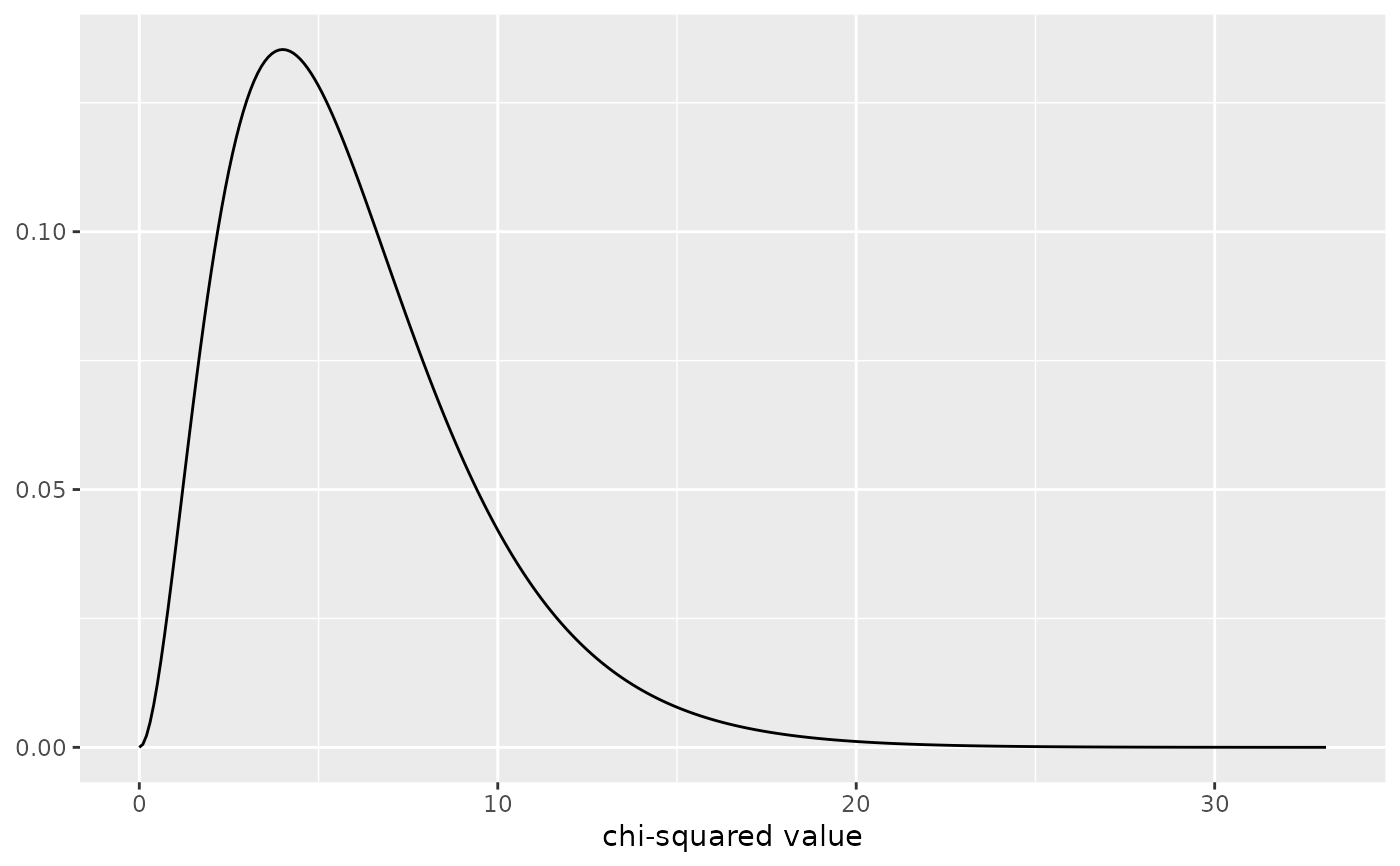
\includegraphics[scale=0.45]{../Figures/fig_chi_square1.png}
			%	\end{subfigure}
	\end{figure}
	
	
\end{frame}

\begin{frame}{Asymptotics for the Normal distribution}
	When $\mu$ and $\sigma$ are unknown and testing the hypothesis
	\begin{equation*}
		H_0 \colon \mu=\mu_0 \quad H_1 \colon \mu \ne \mu_0
	\end{equation*}
	The likelihood ratio is given by
	\begin{equation*}
		\Lambda(x_1,\ldots, x_n)= \left\{ 1+ \frac{1}{n-1}\left( \frac{\overline{x}-\mu_0}{s/\sqrt{n}}\right)\right\}^{-n/2}
	\end{equation*}
	where $s^2= \frac{1}{n-1}\sum_{i}(x_i-\overline{x})^2$. The critical regions are of the form
	\begin{equation*}
		G= \{ (x_1,\ldots, x_n)\in \mathbb{R}^n: \left|\frac{\overline{x}-\mu_0}{s/\sqrt{n}} \right|\ge c\}
	\end{equation*}
\end{frame}
\begin{frame}{$p$-values}
	The test statistic $\frac{\overline{x}-\mu_0}{s/\sqrt{n}}$ is critical to reject $H_0$ or not. The decision procedure is as follows
	\begin{equation*}
		\begin{split}
			\text{if }&\left| \frac{\overline{x}-\mu_0}{s/\sqrt{n}} \right| \ge c \text{ then we assume }H_1\\
			\text{if }&\left| \frac{\overline{x}-\mu_0}{s/\sqrt{n}} \right| <c \text{ then we assume }H_0
		\end{split}
	\end{equation*}
	Furthermore, we have the following equivalence
	\begin{equation*}
		P\left(	\left| \frac{\overline{x}-\mu_0}{s/\sqrt{n}} \right| \ge u \right)\le \alpha \iff u \ge c
	\end{equation*}
	The $p$-value associated with the outcome $u$ of the test statistic $\frac{\overline{x}-\mu_0}{S/\sqrt{n}}$ 
	\begin{equation*}
		P\left(	\left| \frac{\overline{x}-\mu_0}{s/\sqrt{n}} \right| \ge |u| \right)
	\end{equation*}
\end{frame}

\begin{frame}{$p$-values (cont)}
	Thus if an outcome $u$ of $\frac{\overline{x}-\mu_0}{S/\sqrt{n}}$  satisfies 
	\begin{equation*}
		P\left(	\left| \frac{\overline{x}-\mu_0}{s/\sqrt{n}} \right| \ge |u| \right) \le \alpha \text{ we accept }H_1
	\end{equation*}
	
\end{frame}
	
	
	
	%\begin{frame}{Fourier Transform}
	%	\begin{figure}[h]
		%	\centering
		%	%	\begin{subfigure}{0.4\textwidth}
			%		%		\centering
			%		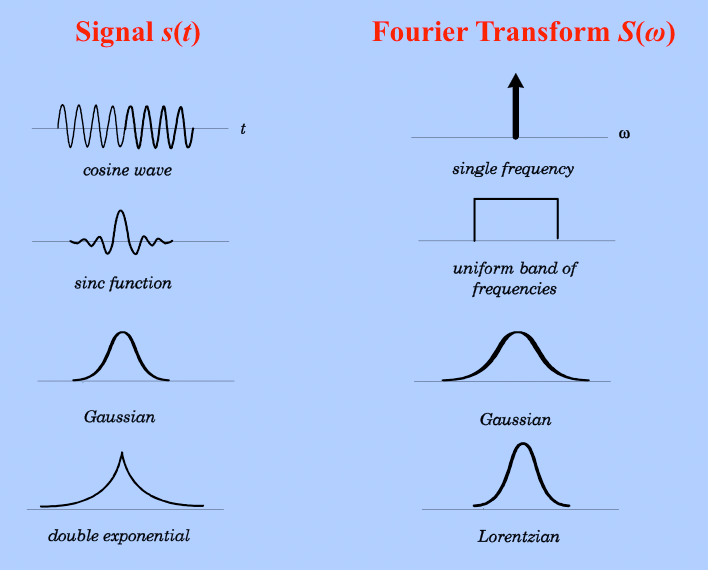
\includegraphics[scale=0.65]{../Figures/fig_fourier_transform.}
			%		%	\end{subfigure}
		%\end{figure}
		%\end{frame}
		
		
\begin{frame}{References}
	Materials and some of the pictures are from \citep{pestman,hogg}.
	
	\printbibliography 	
		
		%	I have used some of the graphs by hacking TiKz code from StakExchange, Inkscape for more aesthetic plots and other old tricks of \TeX
\end{frame}
		
		
	\end{document}
